\documentclass[a4j,twocolumn,10pt]{jsarticle}
%\documentclass{ipsjpapers}
%\makeatletter
%\def\documentstyle#1{}
\pagestyle{empty}
% 画像挿入用パッケージ
\usepackage[dvipdfmx]{graphicx}
\usepackage{url}
%\usepackage{cite}



% 巻数,号数などの設定
%\setcounter{巻数}{41}
%\setcounter{号数}{6}
%\setcounter{volpageoffset}{1234}
%\受付{12}{2}{4}
%\採録{12}{5}{11}

% ユーザが定義したマクロなど.
\makeatletter
%\let\@ARRAY\@array \def\@array{\def\<{\inhibitglue}\@ARRAY}
%\def\<{\(\langle\)}
%\def\>{\(\rangle\)}
%\def\|{\verb|}
%\def\Underline{\setbox0\hbox\input{topic_presentation.tex}
\bgroup\let\\\endUnderline
%\def\endUnderline{\vphantom{y}\egroup\smash{\underline{\box0}}\\}
%\def\LATEX{\iLATEX\Large}
%\def\LATEx{\iLATEX\normalsize}
%\def\LATex{\iLATEX\small}
%\def\iLATEX#1{L\kern-.36em\raise.3ex\hbox{#1\bf A}\kern-.15em
%    T\kern-.1667em\lower.7ex\hbox{E}\kern-.125emX}
%\def\LATEXe{\ifx\LaTeXe\undefined \LaTeX 2e\else\LaTeXe\fi}
%\def\LATExe{\ifx\LaTeXe\undefined \iLATEX\scriptsize 2e\else\LaTeXe\fi}
%\def\Quote{\list{}{}\item[]}
%\let\endQuote\endlist
%\def\TT{\if@LaTeX@e\tt\fi}
%\def\CS#1{\if@LaTeX@e\tt\expandafter\string\csname#1\endcsname\else
%	$\backslash$#1\fi}

\def\section{\@startsection{section}{1}{\z@}{3ex plus .2ex minus .2ex}%
			{.5ex plus .2ex minus .2ex}{\large\bfseries}}
\def\thesection{\arabic{section}.}
\def\subsection{\@startsection{subsection}{1}{\z@}{3ex plus .2ex minus .2ex}%
			{.2ex plus .2ex minus .2ex}{\normalsize\bfseries}}
\def\thesubsection{\arabic{section}.\arabic{subsection}}
\def\subsubsection{\@startsection{subsubsection}{1}{\z@}{2ex plus .2ex minus .2ex}%
			{.2ex plus .2ex minus .2ex}{\normalsize\bfseries}}
\def\thesubsubsection{\arabic{section}.\arabic{subsection}.\arabic{subsubsection}}


%\def\thefootnote{\fnsymbol{footnote}}
\makeatother

\def\baselinestretch{0.850}

\setlength{\textheight}{24.5cm}%297-30-27 - 5
\setlength{\textwidth}{17.0cm}%210-18-18 - 10
%\setlength{\headheight}{0.0in}
\setlength{\headsep}{-0.3in}
\setlength{\oddsidemargin}{-.4cm}%+3
%\setlength{\evensidemargin}{-.9cm}%+3
\setlength{\columnsep}{7mm}

%文章途中に挿入された図表の余白
%\setlength\intextsep{12pt plus 2pt minus 2pt}
%ページ上部の図と図の余白
%\setlength{\floatsep}{9pt plus 2pt minus 0pt}
%ページ上部の図と本文の余白
%\setlength\textfloatsep{20pt plus 2pt minus 4pt}





\renewcommand{\thefootnote}{\arabic{footnote}}

%\checklines	% 行送りを確認する時に使用

\begin{document}%{
\pagestyle{plain}
%\renewcommand{\thepage}{-- \arabic{page} --}
\twocolumn[%
%\begin{center}
\vspace{-0.8cm}
\title{\Large 
ディスプレイを用いた脈波生成手法の検討\\
\vspace{.9ex}
}

\author{藤井敦寛 \vspace{0.3cm} \\
{情報理工学研究科 計算機科学コース 知的インタラクティブシステム研究室}\\
{6611200054-3}\\
{atsuhiro.fujii@iis.ise.ritsumei.ac.jp}}

\date{\hfill}

\maketitle
\thispagestyle{empty}
\pagestyle{empty}
\vspace{-1.5cm}

\vspace{1.0cm}
]




%\setcounter{footnote}{2}
%\footnotetext{http://www.amazon.com/}

\section{研究の背景と目的}
\label{introduction}
健康管理への意識の高まりから,自身の生体情報を記録するウェアラブルデバイスが広く普及している.記録する生体情報は活動量や呼吸数,体温などさまざまな情報があり,心拍数もそのひとつである.心拍数を取得するために用いられる脈波センサは,緑色のLEDを皮膚に照射して,血管を通して反射した光の変化から脈波を計測する光電式容積脈波記録法(PPG)と呼ばれる方式のものが一般的であり,市販のスマートウォッチに導入されている.スマートウォッチのセンサから取得できる心拍データを用いて疲労度を検出する手法を今井ら\cite{fatigue_detection}が提案している.そのほか,Hanら\cite{arrhythmia_detection}はスマートウォッチから取得された脈波データから心房期外収縮(PAC)および,心室性期外収縮(PVC)を検出する手法を提案している.このように,脈波センサから得られるデータを使用した研究は盛んである.

しかしながら,義手やロボットアームなど人工的な身体には血流が存在しないためスマートウォッチを生身の身体と同様に手首に装着して生体情報を計測することはできない.通話やメッセージ,時計などのスマートウォッチの機能や加速度センサやGPSなどのセンサは人工的な身体でも利用できるが,生体情報の計測はできない.このように,人工的な身体において生身の身体で利用できていたインタフェース,デザイン,プロトコルが利用できない問題がある.この問題を解決するには,現状では追加のセンサを計測可能な身体部位に装着して,何からの通信手段を用いてセンサデータを収集する必要がある.しかし,仮に収集したとしても,スマートウォッチが提供するアプリにデータを与えてサービスを利用することはハードルが高いため,スマートウォッチに搭載されているセンサに計測させたい.しかし,計測可能部位にスマートウォッチを装着すると,本来のスマートウォッチとしての機能(時計やディスプレイ表示,タッチ操作)が利用できなくなるため,スマートウォッチ本来の使用形態である手首に装着して脈拍などの生体情報を計測できるようにすることが望ましい.
\par

本研究では,ディスプレイを用いて脈波センサに脈波データを計測させる手法を検討する.ディスプレイの表示を変化させることで任意の脈波データを脈波センサに読み取らせることができれば,義手やロボットアームなどの人工的な身体にスマートウォッチを装着する場合でも,身体と義手の接合部などで計測された脈波を入力することで,その値をスマートウォッチに読み取らせることができ,スマートウォッチが提供する機能を生身の身体と同様に利用できる.また,人工的な身体にディスプレイを搭載するのみでスマートウォッチには手を加えないため,市販のスマートウォッチをそのまま利用できる.このほか,遠隔地のロボットアバタに適用すれば,操作者の生体情報をアバタの身体でも計測できるようになる.本稿では,ディスプレイによる脈波生成の予備段階として,あらかじめ収集された実際の脈波データを参考にして,ディスプレイの色調を変化させることで,任意の心拍数を計測させる手法を提案する.ディスプレイを用いて脈波センサに脈波データを計測させることができるかを確認し,提案手法の有効性を明らかにする.
\par





\section{予備実験}
\label{preliminary}
\subsection{データ収集}
事前に実際の脈波データを20代男性1名から収集した.図\ref{fig:sensors}の左図に示すように,左手人差し指に光電式容積脈波記録法の脈波センサ(pulsesensor.com製)を装着した.脈波センサはArduinoUNOを介してPCに接続しており,サンプリング周波数は約90Hzで10秒間データの収集を行った.

\subsection{実験方法}
データ収集で使用したPCとは異なるPC(SurfaceLaptop)のディスプレイの色調を変化させた.図\ref{fig:sensors}の右図に示すように,ディスプレイ上に脈波センサを乗せ,光が入らないように布で覆ったあと,ガムテープで固定した.事前に脈波データを収集したときと同じ条件でデータの取得を行った.ディスプレイの色調の変化にはJavaScriptを使用し,ブラウザの背景色を変化させることで制御した.事前に収集した脈波データを1サンプルずつ読み込み,その値に応じた3色で表示を繰り返す.全サンプルの処理が終了した場合,同じデータで再び処理を行う.
\par

表示する色は,次式により定義した.
\begin{equation}
	\label{eqn:low}
	value < \theta_{1} \quad (\theta_{1}=465)
\end{equation}

\begin{equation}
	\label{eqn:middle}
	\theta_{1} \leq value \leq \theta_{2} \quad (\theta_{1}=465, \theta_{2}=685)
\end{equation}

\begin{equation}
	\label{eqn:high}
	\theta_{2} < value \quad (\theta_{2}=685)
\end{equation}
式\ref{eqn:low}を満たす場合はR:150, G:19, B:20,式\ref{eqn:middle}を満たす場合はR:157, G:26, B:27,式\ref{eqn:high}を満たす場合はR:156, G:25, B:26で表現される色を表示する.また,1サンプルを読み込み,色を表示するごとに10msの遅延を挟んだ.

\begin{figure}[!t]
	\begin{center}
		\includegraphics[width=1\linewidth]{figures/sensors.eps}
	\end{center}
	\caption{脈波データの取得方法}
	\label{fig:sensors}
\end{figure}


\subsection{結果と考察}
取得された脈波データを,最初のピークから5秒間切り出した結果を図\ref{fig:pulse}に示す.結果から,ピークを生成できていることが確認できる.したがって,ディスプレイを使用するアプローチは有効だといえる.しかしながら,ピークの位置や値に違いが見られる.これは,ディスプレイ制御の開始時刻とセンサ値の取得の開始時刻を同期していなかったことや,サンプルの処理ごとの遅延を10msに固定していたことが影響したと考えられる.

\begin{figure}[!t]
	\begin{center}
		\includegraphics[width=1\linewidth]{figures/pulse.eps}
	\end{center}
	\caption{脈波センサの取得値の変化}
	\label{fig:pulse}
\end{figure}


\section{今後}
\label{future_work}
予備実験の結果から,ディスプレイを用いて脈波センサに脈波を計測させることができることを確認した.今後は実環境での使用を想定して,身体部位から得られた実際の脈波データを入力することで,ディスプレイ上に設置した脈波センサに同一のデータを計測させる機構を実装する.この機構の想定を図\ref{fig:future_work}に示す.実現するには,ディスプレイに表示する色を自動で決定し続ける必要がある.そのため,脈波データを入力することでディスプレイに表示する色を出力することができるような識別モデルを構築する.

\begin{figure}[!t]
	\begin{center}
		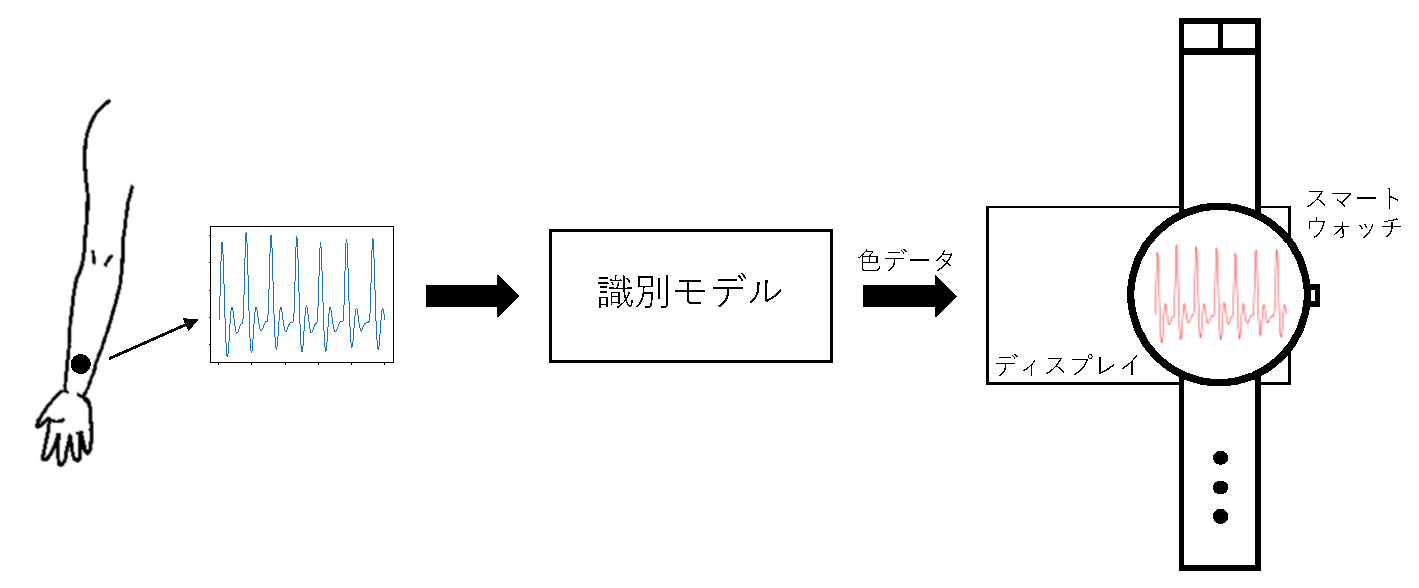
\includegraphics[width=1\linewidth]{figures/future_work.eps}
	\end{center}
	\caption{脈波センサの取得値の変化}
	\label{fig:future_work}
\end{figure}


\section{まとめ}
\label{conclude}
本研究では,ディスプレイを用いて脈波センサに脈波データを計測させる手法を実現するために,ディスプレイの色調を変化させることで,脈波センサの取得値を意図的に操作することが可能であるか調査した.予備実験として,事前に被験者1人から実際の脈波データを収集しておき,そのデータから値に応じた色調をディスプレイに繰り返し表示しながら,ディスプレイ上に設置した脈波センサからデータを取得した.予備実験の結果,ディスプレイ上の脈波センサからピークの存在するデータが取得できた.この結果から,脈波データを計測させるためにディスプレイを用いるアプローチは有効であることが確認できた.
\par

今後は,身体部位から取得された実際の脈波データを,ディスプレイを用いて再現する機構を実装する.そのためには,自動でディスプレイの色調を決定していく必要があるため,適切な識別モデルを設計していく.



\bibliography{references}
\bibliographystyle{junsrt}

\end{document}
